\section{Individual I4.0 Maturity Model}

To enable an individual \ac{I4.0} strategy and applicable guidance, the section-specific frameworks and emphases provide for relevant information and progress in the respective section. One key element is missing to make this orientation lead to an individual strategy to get \ac{I4.0} processes implemented in the organization of the reader of this paper: The competitive environment or rather the benchmark against others in this specific industry combined with the individual state of digitalization. To solve this, we collated insights to outline the individual maturity model. The objective is to receive an individual scheme on a strategic level, industry-specific and connected to the status quo of the considered organization \& competition, to implement relevant and effective \ac{I4.0} processes and ultimately transform to sustainable solutions.

The following maturity model insights are the basis for the \ac{II4.0MM}, but are either only focusing on manufacturing-specific \ac{I4.0} or not aggregating all relevant data

\begin{enumerate}
\item Industry 4.0 Maturity Model \cite{Schumacher2016161}
\item The Connected Enterprise Maturity Model \cite{RockWellAutomation-connectedEnterpriseMaturityModel}
\item The Digital Advantage: How digital Leaders outperform their peers in every industry \cite{CapgeminiMaturityModelDigitalAdvantage}
\end{enumerate}

The \ac{II4.0MM} is structured into 3 steps, which are described subsequently, enriched with the appropriate frameworks and studies.


\begin{figure}[H]
\centering
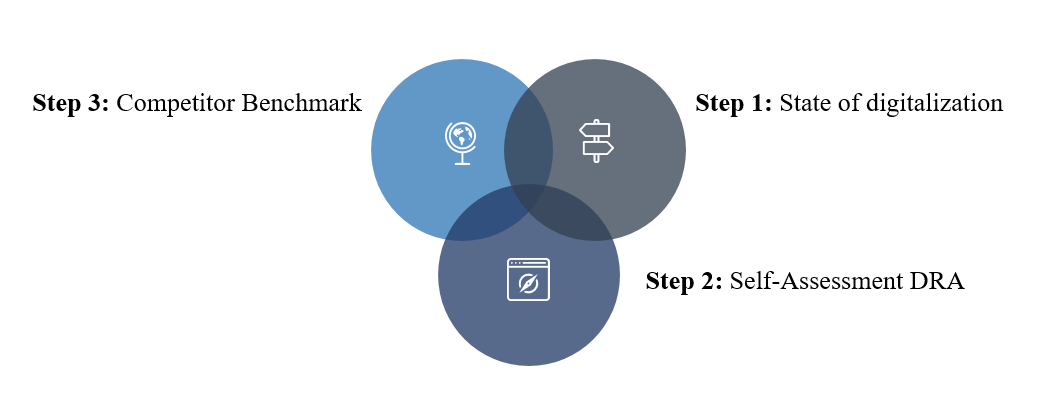
\includegraphics[width=1\columnwidth]{images/II40MM_grafik.PNG}
\caption{\ac{II4.0MM} 3 steps: State of digitalization, Self-Assessment (DRA), Competitor Benchmark}
\end{figure}

It is important to define what is meant with the term \emph{\ac{II4.0MM}}. In this paper, we combine the three key aspects of the state of digitalization, which are described in chapter \emph{2.2} %TODO kann man das hier irgendwie noch besser darstellen mit der Referenz zum vorherigen Kapitel im Paper? %
with self-assessment tools to get the benchmark of the competition in the considered industry to shape an applicable model. This can be used to get strategic leaders converted to implement digital and \ac{IoT} processes in their respective organization.
Other studies may call it \emph{digital Readiness}, which is not focusing on \ac{I4.0} or \ac{DT} in detail.

The first step of the \ac{II4.0MM} is to determine the state of digitalization. A quick hint is delivered by the four Types of Digital Maturity by \cite[p.4]{CapgeminiMaturityModelDigitalAdvantage}:

\begin{figure}[H]
\centering
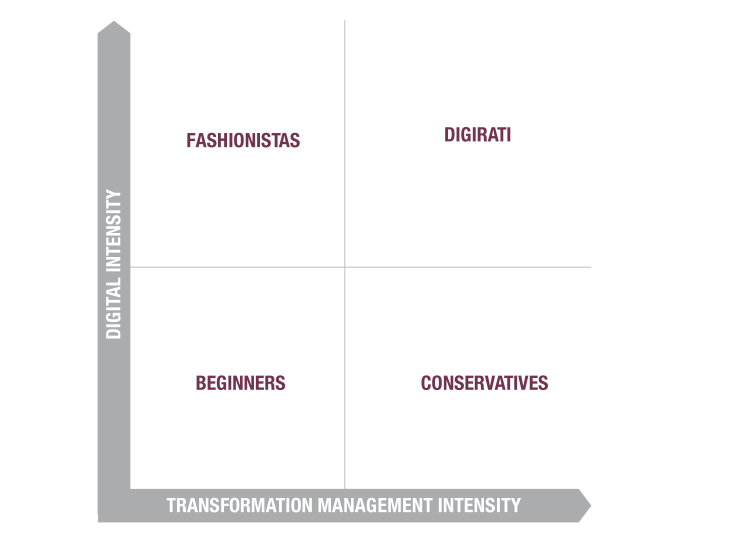
\includegraphics[width=1\columnwidth]{images/maturityModel_4segments_capgemini.PNG}
\caption{Four Types of Digital Maturity: Fashionistas, Digirati, Beginners, Conservatives \cite{CapgeminiMaturityModelDigitalAdvantage}}
\end{figure}

Those four types are distinguished by the affiliation to two dimensions: digital intensity (technology-enabled initiatives) and transformation management intensity (leadership capability) \cite{CapgeminiMaturityModelDigitalAdvantage}. Extending those dimensions with the business models as the third key aspects of the state of digitalization, we can see an analogy to our predefined model.

Every organization can classify themselves into one described type by answering specific questionnaires or deploy a \ac{DRA} \cite{Schumacher2016161} \cite{ReadinessIndustrie40Impulse} \cite{i40-self-assessment-PwC:2016}. After the first segmentation it is recommended to establish a connection to individual competition benchmark. This is the second step of the \ac{II4.0MM}. General information can be found in our chapter 3 \emph{Sector specific application of frameworks} and the respective recommended frameworks with further information. The \ac{II4.0MM} cannot deliver further benchmark information but the urgency of transformation can be explorated via the following resources:
\begin{enumerate}
\item Digital Readiness Assessment: Does your business strategy work in a digital world? \cite{ey-dra}
\item IMPULS – Industrie 4.0 Readiness \cite{ReadinessIndustrie40Impulse}
\item Industry 4.0 Self Assessment \cite{i40-self-assessment-PwC:2016}
\end{enumerate}

This step concludes the \ac{II4.0MM} and delivers a scheme, which can be used for \ac{I4.0} implementation in the individual context.
